% This LaTeX was auto-generated from MATLAB code.
% To make changes, update the MATLAB code and export to LaTeX again.

\documentclass{article}

\usepackage[utf8]{inputenc}
\usepackage[T1]{fontenc}
\usepackage{lmodern}
\usepackage{graphicx}
\usepackage{color}
\usepackage{hyperref}
\usepackage{amsmath}
\usepackage{amsfonts}
\usepackage{epstopdf}
\usepackage[table]{xcolor}
\usepackage{matlab}

\sloppy
\epstopdfsetup{outdir=./}
\graphicspath{ {./Lab08_images/} }

\begin{document}

\matlabtitle{LAB 8: FREQUENCY DOMAIN IDENTIFICATION OF QNET DC MOTOR}

\begin{matlabcode}
%---------------------------------------
% Fill in your student Name and ID.
Students.Name = 'Seyed Yazdan Zinati';
Students.ID = '260928077';
%---------------------------------------
\end{matlabcode}


\matlabheading{\textbf{0. Objectives}}

\begin{par}
\begin{flushleft}
In this lab, we will use frequency analysis to identify the transfer function of the Virtual Motor. To initiate a connection with the virtual motor, run the following:
\end{flushleft}
\end{par}

\begin{matlabcode}
Motor = VirtualMotor();
\end{matlabcode}


\matlabheading{\textbf{1. Frequency Response Analysis}}

\begin{par}
\begin{flushleft}
When a cosine wave $x(t)=M_x \cos (\omega t)$ is injected into a linear system, the system will respond with the same frequency $\omega$, a certain magnitude $M_x$ and a certain phase angle relative to the input $\phi$. The steady-state system output can be written as $y(t)=M_y \cos (\omega t+\phi )$.
\end{flushleft}
\end{par}

\begin{par}
\begin{flushleft}
If $G(j\omega )$ is the frequency response of this system, we define the magnitude and phase at $\omega$ by:
\end{flushleft}
\end{par}

\begin{par}
$$M(\omega )=\frac{M_y }{M_x }=||G(j\omega )||$$
\end{par}

\begin{par}
$$\phi (\omega )=\angle G(j\omega )$$
\end{par}

\matlabheading{\textit{1.1 Bode plot}}

\begin{par}
\begin{flushleft}
The Bode plot presents the magnitude and the phase shift between the input and output at each frequency. It is possible to draw a \texttt{point-by-point} Bode plot by injecting a cosine wave with a known frequency, once at a time, and measuring the magnitude and phase shift of the output after it reaches its steady-state.
\end{flushleft}
\end{par}

\begin{par}
\begin{flushleft}
In a bode plot the magnitude is represented in a logarithmic scale in decibels (db).
\end{flushleft}
\end{par}

\begin{par}
$$M_{db} (\omega )=20\log (M(\omega ))$$
\end{par}

\begin{par}
\begin{flushleft}
The phase at each frequency can be found by measuring the temporal delay between the output and the input when the input is a cosine wave. Another way to measure the phase shift is through the Lissajous method. A Lissajous curve (an ellipsoid) is found when we try to plot the output in function of the input (XY plot). In fact, we can show that at a frequency $\omega$
\end{flushleft}
\end{par}

\begin{par}
$$\cos (\phi )=\frac{y^* }{M_y }$$
\end{par}

\begin{par}
\begin{flushleft}
Where $y^*$ is the value of the output $y$ when the input $x$ is at the maximum $M_x$.
\end{flushleft}
\end{par}

\begin{par}
\begin{flushleft}
An illustration of using the Lissajous method (taken from Wikipedia) is shown below:
\end{flushleft}
\end{par}

\begin{par}
\begin{flushleft}
\textless{}\textless{}fig\_lab08\_lissajousphase.png\textgreater{}\textgreater{}
\end{flushleft}
\end{par}

\matlabheading{\textit{Question 1 (2.5 mark)}}

\begin{itemize}
\setlength{\itemsep}{-1ex}
   \item{\begin{flushleft} Define the following transfer function in \texttt{\textbf{MATLAB}} \end{flushleft}}
\end{itemize}

\begin{par}
$$G(s)=\frac{s+4}{s^2 +s+1}$$
\end{par}

\begin{matlabcode}
s = tf('s');
G = (s + 4)/(s^2 + s + 1)
\end{matlabcode}
\begin{matlaboutput}
G =
 
     s + 4
  -----------
  s^2 + s + 1
 
Continuous-time transfer function.
\end{matlaboutput}


\begin{itemize}
\setlength{\itemsep}{-1ex}
   \item{\begin{flushleft} Plot the bode graph of this system. (Hint: help \texttt{\textbf{bode}}) \end{flushleft}}
\end{itemize}

\begin{matlabcode}
figure(1); clf;

bode(G)

grid on
\end{matlabcode}
\begin{center}
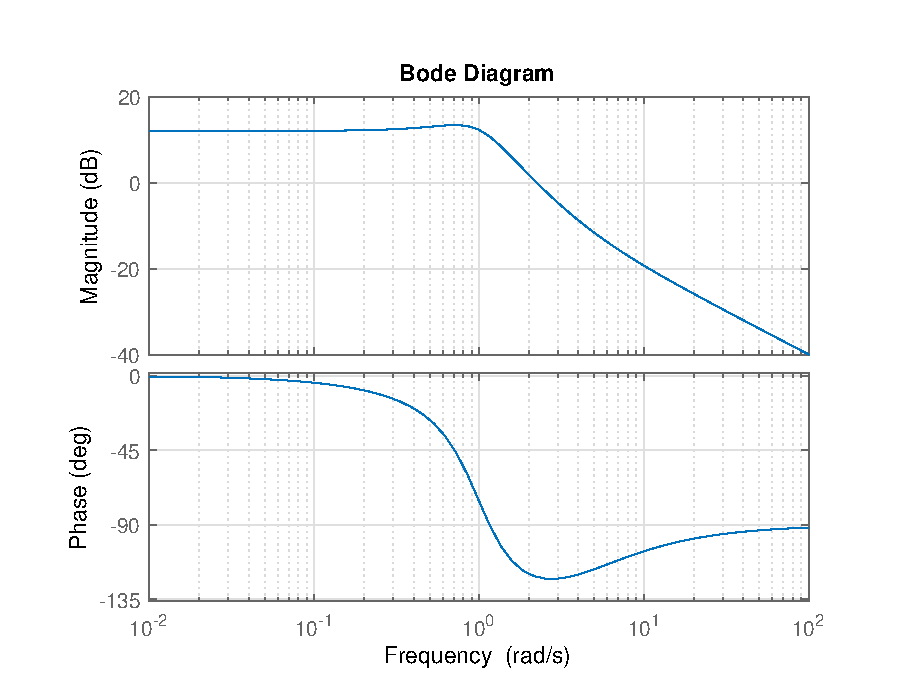
\includegraphics[width=\maxwidth{56.196688409433015em}]{figure_0.eps}
\end{center}


\begin{itemize}
\setlength{\itemsep}{-1ex}
   \item{\begin{flushleft} Consider the following signal: \end{flushleft}}
\end{itemize}

\begin{matlabcode}
rng(datetime('now').Year*randi([1,20],1))
Freq = round(0.1+rand(1), 2);
t = 0:0.01:round(10/Freq);
x = cos(2*pi*Freq*t);
\end{matlabcode}


\begin{par}
\begin{flushleft}
Using \texttt{\textbf{lsim}} simulate the output $y(t)$ representing the response of the system $G$ to the signal $x(t)$.
\end{flushleft}
\end{par}

\begin{matlabcode}
y = lsim(G, x, t);

figure(2); clf;
title(sprintf('Student %d - Freq %3.2f Hz - Phase %+03d deg - Magnitude %4.2f',...
    Students.ID(1), Freq, round(180*angle(evalfr(G, 2*pi*Freq*1i))/pi), abs(evalfr(G, 2*pi*Freq*1i))));
hold on
plot(t, x)
plot(t, y)
grid on
legend('x', 'y')
\end{matlabcode}
\begin{center}
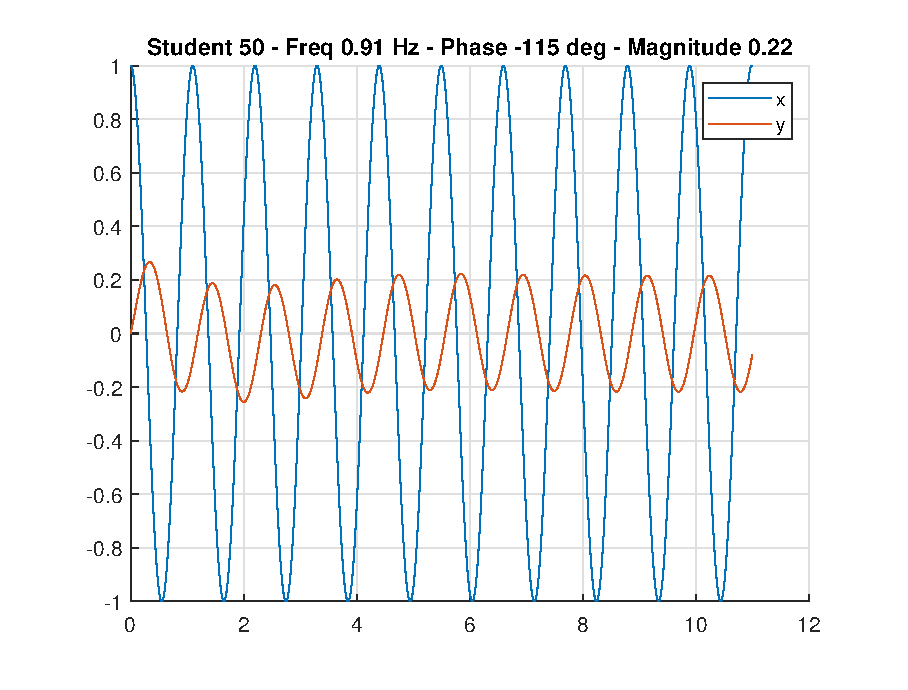
\includegraphics[width=\maxwidth{56.196688409433015em}]{figure_1.eps}
\end{center}


\begin{itemize}
\setlength{\itemsep}{-1ex}
   \item{\begin{flushleft} Plot $y(t)$ in function of $x(t)$. \end{flushleft}}
\end{itemize}

\begin{matlabcode}
figure(3); clf;

plot(x, y)

title(sprintf('Student %d - XY Plot', Students.ID(1)));
grid on
\end{matlabcode}
\begin{center}
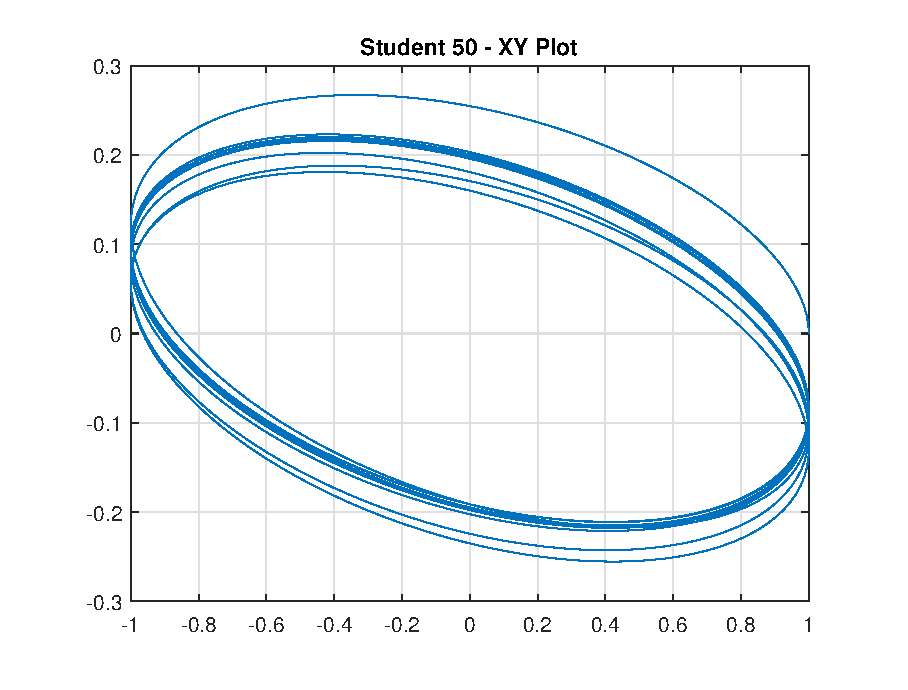
\includegraphics[width=\maxwidth{56.196688409433015em}]{figure_2.eps}
\end{center}


\begin{itemize}
\setlength{\itemsep}{-1ex}
   \item{\begin{flushleft} Find graphically the phase $\phi$ and magnitude $M$ at the specified frequency. \end{flushleft}}
\end{itemize}

\begin{matlabcode}
showMyAndYStar(t, x, y, Freq);
\end{matlabcode}
\begin{center}
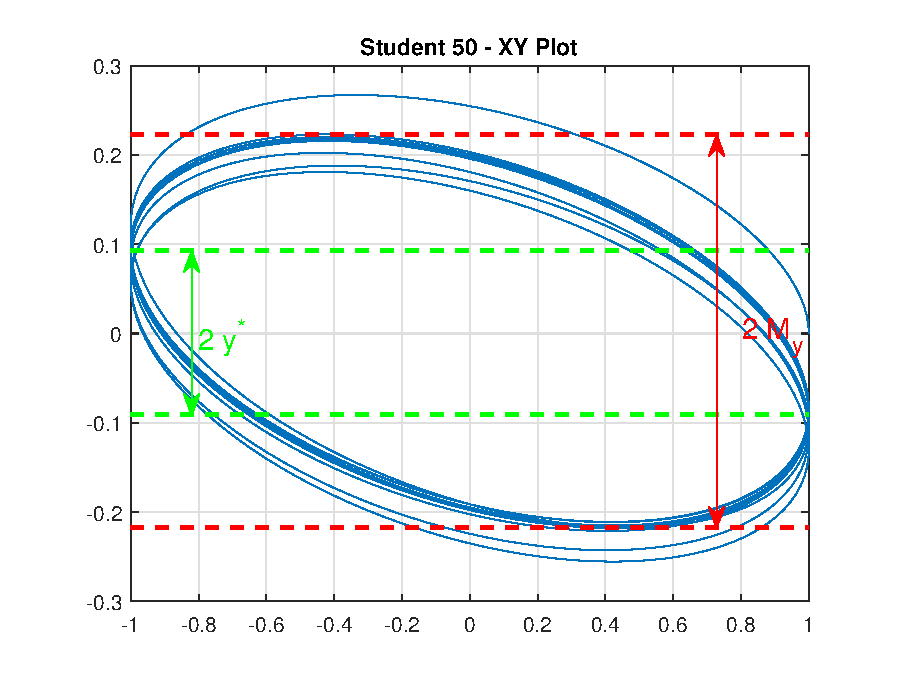
\includegraphics[width=\maxwidth{56.196688409433015em}]{figure_3.eps}
\end{center}
\begin{matlabcode}
y_star = (0.07003 - (-0.07043)) / 2;
M_y = (0.1883 - (-0.1845)) / 2;

% phase
cos_phi = y_star / M_y;
phi = -180 + acosd(cos_phi)
\end{matlabcode}
\begin{matlaboutput}
phi = -112.1338
\end{matlaboutput}
\begin{matlabcode}

% magnitude
M = 2*M_y / (0.451185 + 0.434345)
\end{matlabcode}
\begin{matlaboutput}
M = 0.4210
\end{matlaboutput}


\matlabheading{\textbf{3. Identification of Qnet DC Motor Frequency Response}}

\begin{par}
\begin{flushleft}
To avoid the non-linear domain of the DC Motor at low voltage we will stimulate the DC Motor with offsetted cosine waves. We choose the following voltage signal:
\end{flushleft}
\end{par}

\begin{par}
$$v(t)=4+2\cos (2\pi ft)$$
\end{par}

\begin{par}
\begin{flushleft}
To send a cosine wave of frequency $f=0.5$ Hz to the Virtual Motor we do the following:
\end{flushleft}
\end{par}

\begin{matlabcode}
dt = 0.01; % sampling time
T = 15; % simulation duration
t = 0:dt:T; % define the time signal
vAmp = 2; % cosine amplitude
vOffset = 4; % voltage offset
Freq = 0.5; % frequency of cosine wave
Motor.reset();
Motor.input(vOffset + vAmp * cos(2*pi*Freq*t));
Motor.off();
Motor.save(Students, 'Lab08.Sinewave');
Motor.load('Lab08.Sinewave');
\end{matlabcode}
\begin{matlaboutput}
VirtualMotor::load::info: Recovering data collected by students: [260928077] .
\end{matlaboutput}


\begin{par}
\begin{flushleft}
For frequency analysis we are only interested at the steady-state response. We can retrieve the resulting angular velocity at steady state by:
\end{flushleft}
\end{par}

\begin{matlabcode}
delay = 5; % Ignore the first 5 seconds of experiment (transient response)
w = Motor.velocity(t >= delay); 
v = Motor.voltage(t >= delay);
\end{matlabcode}


\begin{par}
\begin{flushleft}
The following shows a plot of the temporal response.
\end{flushleft}
\end{par}

\begin{matlabcode}
figure(4), clf;
subplot(2, 1, 1);
plot(t(t >= delay), v, 'r', 'linewidth', 2.0);
legend('Voltage (V)')
grid on
xlim([delay, T])
title(sprintf('Student %d - Voltage and Angular velocity', Students.ID(1)));
subplot(2, 1, 2);
plot(t(t >= delay), w, 'b', 'linewidth', 2.0);
legend('Angular velocity (rad/s)')
grid on
xlim([delay, T])
\end{matlabcode}
\begin{center}
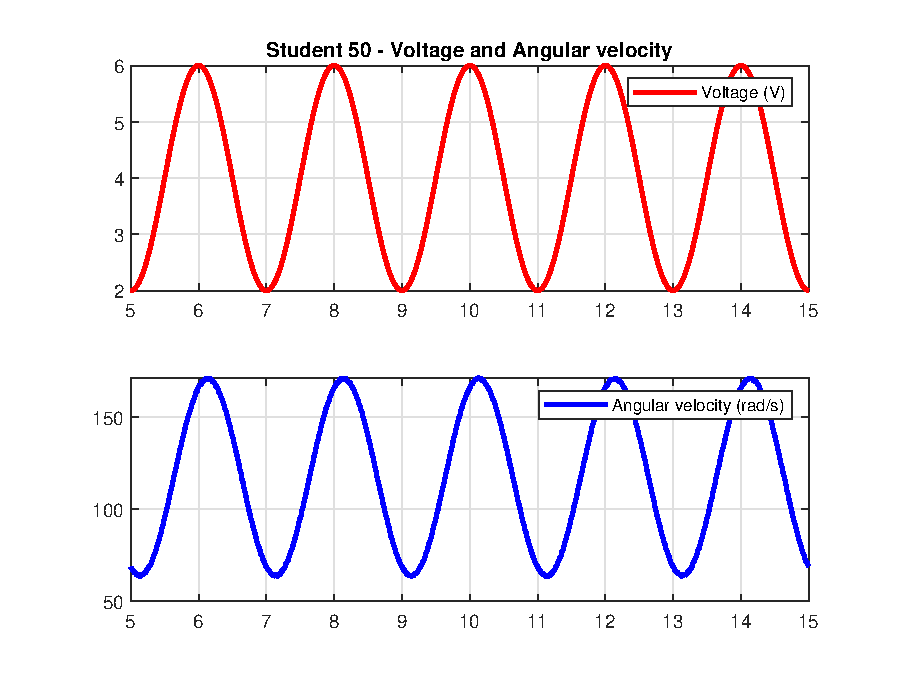
\includegraphics[width=\maxwidth{56.196688409433015em}]{figure_4.eps}
\end{center}


\begin{par}
\begin{flushleft}
And the following shows the XY plot, which we can use to find $y^*$,  $M_y$ and $M_x$.
\end{flushleft}
\end{par}

\begin{matlabcode}
w_filter = medfilt1(w, 10, 'truncate'); % we can filter the noise if needed

figure(5), clf; hold on;
title(sprintf('Student %d - Voltage vs Angular velocity', Students.ID));
plot(v, w_filter, 'k');
grid on
xlabel('Voltage (V)')
ylabel('Angular velocity (rad/s)')
xlim([2 6])
\end{matlabcode}
\begin{center}
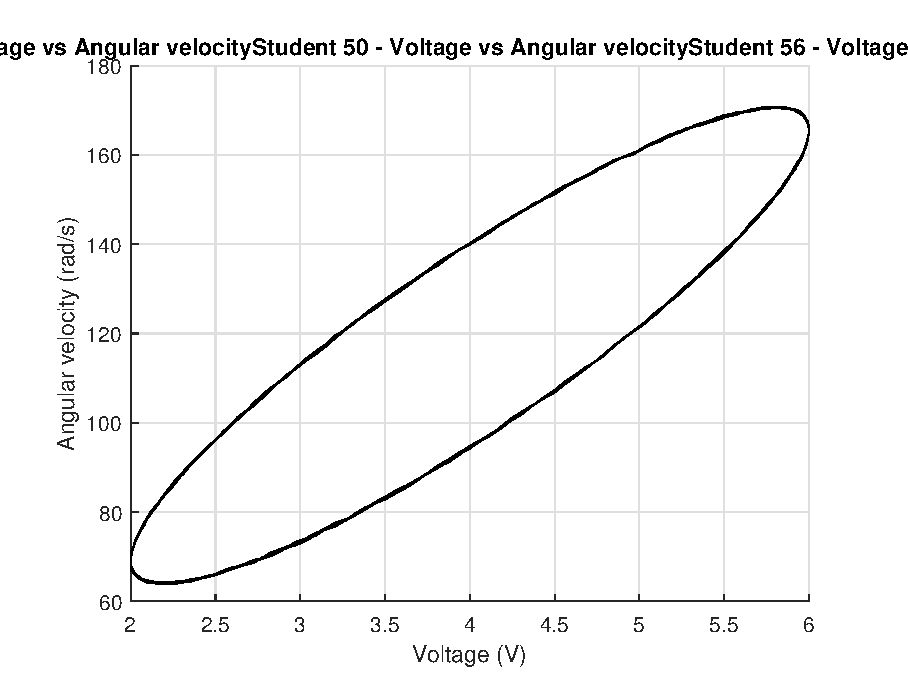
\includegraphics[width=\maxwidth{56.196688409433015em}]{figure_5.eps}
\end{center}


\matlabheading{\textit{Question 3 (3.0 marks)}}

\begin{par}
\begin{flushleft}
Find the magnitude and phase of the transfer function of the Virtual Motor for the following frequencies.
\end{flushleft}
\end{par}

\begin{matlabcode}
FreqVect = [0.05, 0.1, 0.2, 0.4, 0.6, 0.8, 1.0, 1.2, 2.0, 4.0, 6.0];

dt = 0.01;  % sampling time
T = 15; % simulation duration
t = 0:dt:T;  % define the time signal
vAmp = 2  % cosine amplitude
\end{matlabcode}
\begin{matlaboutput}
vAmp = 2
\end{matlaboutput}
\begin{matlabcode}
vOffset = 4  % voltage offset
\end{matlabcode}
\begin{matlaboutput}
vOffset = 4
\end{matlaboutput}
\begin{matlabcode}
Freq = 6  % frequency of cosine wave (a frequency from FreqVect)
\end{matlabcode}
\begin{matlaboutput}
Freq = 6
\end{matlaboutput}
\begin{matlabcode}
Motor.reset();
Motor.input(vOffset + vAmp * cos(2*pi*Freq*t));
Motor.off();
Motor.save(Students, 'Lab08.Sinewave');
Motor.load('Lab08.Sinewave');
\end{matlabcode}
\begin{matlaboutput}
VirtualMotor::load::info: Recovering data collected by students: [260928077] .
\end{matlaboutput}
\begin{matlabcode}

delay = 5; % Ignore the first 5 seconds of experiment (transient response)
w = Motor.velocity(t >= delay); 
v = Motor.voltage(t >= delay);
w_filter = medfilt1(w, 10, 'truncate'); % we can filter the noise if needed

figure(6), clf; hold on;
title(sprintf('Student %d - Voltage vs Angular velocity', Students.ID));
plot(v, w_filter, 'k');
grid on
xlabel('Voltage (V)')
ylabel('Angular velocity (rad/s)')
xlim([2 6])
\end{matlabcode}
\begin{center}
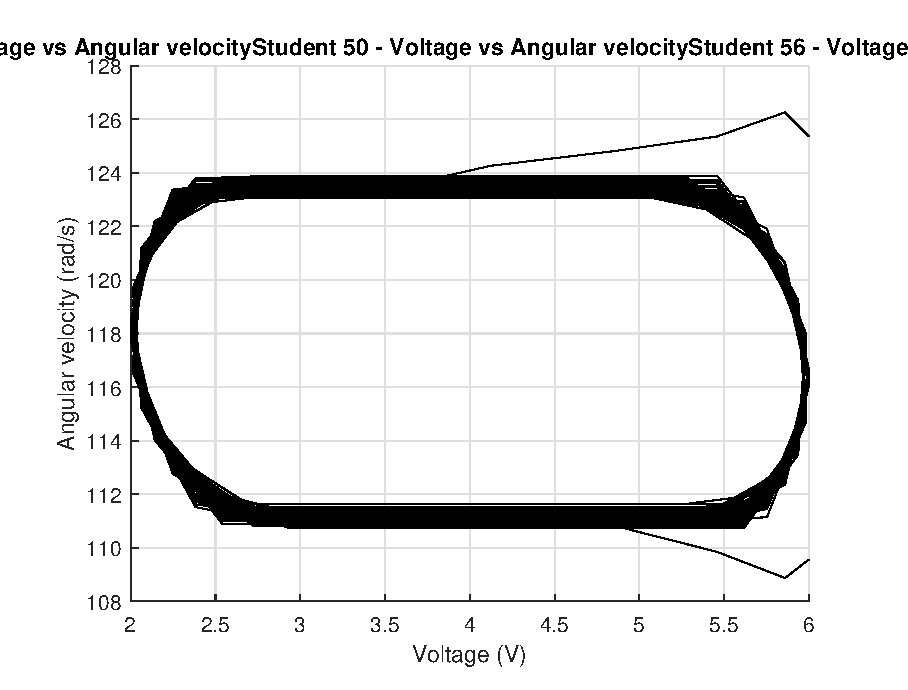
\includegraphics[width=\maxwidth{56.196688409433015em}]{figure_6.eps}
\end{center}


\begin{par}
\begin{flushleft}
Measure graphically the phase and magnitude for each frequency and put it here. Note: The size of MagnitudeDB and PhaseDeg is the same as FreqVect.
\end{flushleft}
\end{par}

\begin{matlabcode}
% Answer here
% 20*log10(M) we get: 
MagnitudeDB = [35.12, 35.24, 35.16, 34.79, 34.19, 33.43, 33.24, 32.34, 29.72, 21.12, 16.24];
PhaseDeg = - [2.75, 5.35, 10.5, 20.46, 29.56, 38.2, 42.9, 50.43, 68.2, 89.53, 90 ];
\end{matlabcode}


\matlabheading{\textit{Question 4 (1.0 mark)}}

\begin{par}
\begin{flushleft}
Draw the resulting Bode plot (Magnitude (dB) vs Frequency (Hz)) on a semilog plot and Phase (deg) vs Frequency (Hz) on a semilog plot). (Hint: help \texttt{\textbf{semilogx}})
\end{flushleft}
\end{par}

\begin{matlabcode}
omega = 2 * pi * FreqVect;
figure(7); clf;
subplot(2, 1, 1)
% Draw magnitude here
semilogx(omega,MagnitudeDB)
grid on
subplot(2, 1, 2)
% Draw Phase here
semilogx(omega,PhaseDeg)
grid on
\end{matlabcode}
\begin{center}
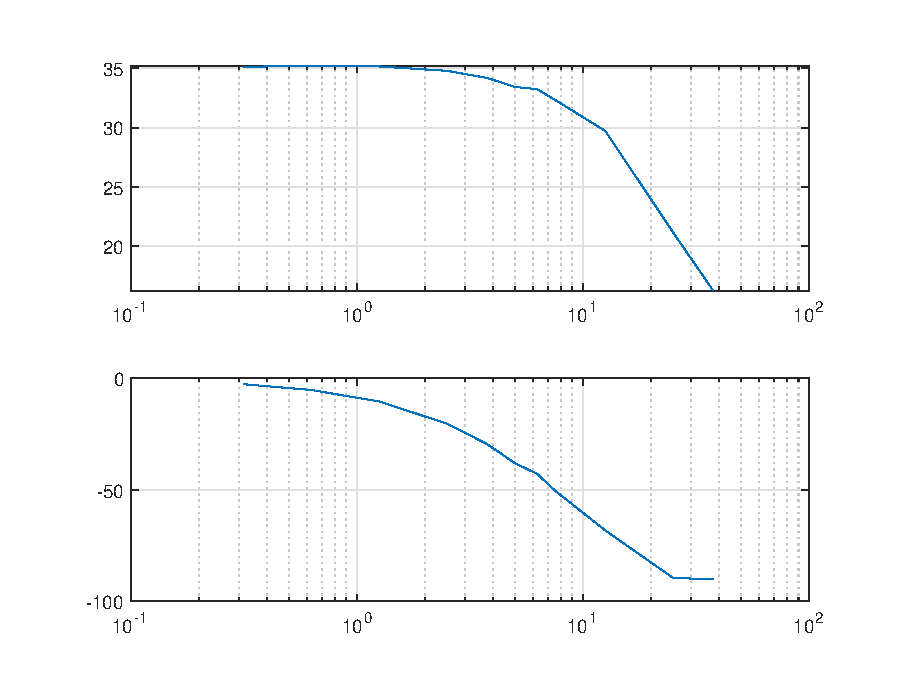
\includegraphics[width=\maxwidth{56.196688409433015em}]{figure_7.eps}
\end{center}


\matlabheading{\textit{Question 5 (1.0 mark)}}

\begin{par}
\begin{flushleft}
From the Bode plot, measure the DC gain.
\end{flushleft}
\end{par}

\begin{matlabcode}
DC_gain = 10^(35.12/20)
\end{matlabcode}
\begin{matlaboutput}
DC_gain = 57.0164
\end{matlaboutput}


\matlabheading{\textit{Question 6 (1.0 mark)}}

\begin{par}
\begin{flushleft}
From the Bode plot, measure the cut-off frequency (Frequency at which the magnitude drops by a factor of $-20\log_{10} \left({{\frac{1}{\sqrt{2}}}}\right)=-3$ (dB) from the DC gain).
\end{flushleft}
\end{par}

\begin{matlabcode}
w_cutoff = 8.09342
\end{matlabcode}
\begin{matlaboutput}
w_cutoff = 8.0934
\end{matlaboutput}


\matlabheading{\textit{Question 7 (1.5 mark)}}

\begin{par}
\begin{flushleft}
For a first order system the transfer function is expressed by
\end{flushleft}
\end{par}

\begin{par}
$$H(s)={{\frac{DC_{gain} }{1+{{\frac{s}{\omega_{cutoff} }}}}}}$$
\end{par}

\begin{itemize}
\setlength{\itemsep}{-1ex}
   \item{\begin{flushleft} Write the transfer function of the identified DC Motor. \end{flushleft}}
\end{itemize}

\begin{matlabcode}
H =  DC_gain / (1 + (s/w_cutoff))
\end{matlabcode}
\begin{matlaboutput}
H =
 
    461.5
  ---------
  s + 8.093
 
Continuous-time transfer function.
\end{matlaboutput}


\begin{itemize}
\setlength{\itemsep}{-1ex}
   \item{\begin{flushleft} Complete the code to superpose the experimental bode plot with the bode plot of the identified transfer function. \end{flushleft}}
\end{itemize}

\begin{matlabcode}
H_Freq = squeeze(freqresp(H, omega, 'rad/s'))';


H_MagnitudeDB =  20*log10(abs(H_Freq)) % find magnitude in db
\end{matlabcode}
\begin{matlaboutput}
H_MagnitudeDB = 1x11    
   35.1135   35.0939   35.0165   34.7202   34.2672   33.7032   33.0715   32.4065   29.7915   24.8493   21.5603

\end{matlaboutput}
\begin{matlabcode}
H_PhaseDeg =  -rad2deg(angle(H_Freq)) % find phase in degrees
\end{matlabcode}
\begin{matlaboutput}
H_PhaseDeg = 1x11    
   -2.2229   -4.4392   -8.8256  -17.2513  -24.9761  -31.8430  -37.8234  -42.9719  -57.2163  -72.1500  -77.8834

\end{matlaboutput}
\begin{matlabcode}

figure(9)
subplot(211)
semilogx(omega, [MagnitudeDB; H_MagnitudeDB])
grid on
subplot(212)
semilogx(omega, [PhaseDeg; H_PhaseDeg])
grid on
\end{matlabcode}
\begin{center}
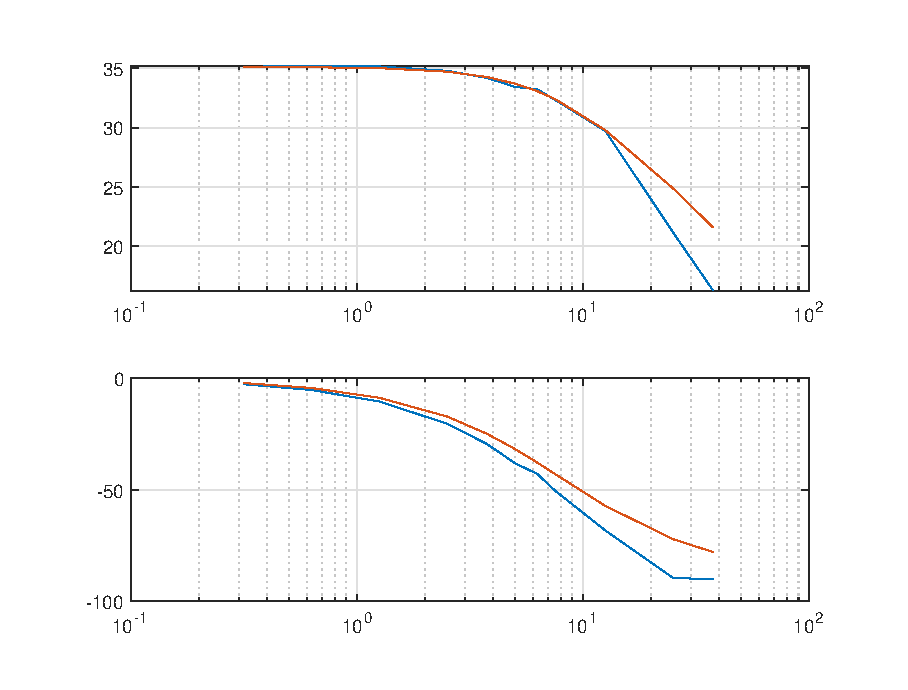
\includegraphics[width=\maxwidth{56.196688409433015em}]{figure_8.eps}
\end{center}


\begin{itemize}
\setlength{\itemsep}{-1ex}
   \item{\begin{flushleft} How accurate is the point-by-point bode plot for high frequencies? Comment on your results. \end{flushleft}}
\end{itemize}

\begin{matlabcode}
% The point-by-point bode plot is quite accurate when working 
% with small frequencies, it becomes less accurate for higher frequencies.
% This can bee seen as the phase and magnitude don't exactly superpose.
% This is due to the fact that the accuracy is inversly proportional to the
% thickness of the curve. Therefore: as we increase the frequency, the thickness of
% the curve increases, and our accuracy drops.
\end{matlabcode}


\matlabheading{\textbf{4. Useful Functions}}

\matlabheading{\textit{4.1 Customize the XY plot}}

\begin{matlabcode}
function showMyAndYStar(t, x, y, Freq)
max_y = max(y(t > round(5/Freq)));
max_x = max(x(t > round(5/Freq)));
min_y = min(y(t > round(5/Freq)));
min_x = min(x(t > round(5/Freq)));
star_y_1 = mean(y(t > round(5/Freq) & abs(x-max_x) < 0.05));
star_y_2 = mean(y(t > round(5/Freq) & abs(x-min_x) < 0.05));

gcf; hold on; axPos = get(gca, 'Position'); xMinMax = xlim; yMinMax = ylim;
plot([min_x, max_x], [max_y, max_y], '--r', 'linewidth', 2.0)
plot([min_x, max_x], [min_y, min_y], '--r', 'linewidth', 2.0)
annotation('doublearrow', [0.8, 0.8],...
    axPos(2)+(([max_y, min_y] - yMinMax(1)) / (yMinMax(2) - yMinMax(1)))*axPos(4), 'Color', 'red')
text(0.8, 0.0, '2 M_y', 'Color', 'red', 'FontSize', 14)
plot([min_x, max_x], [star_y_1, star_y_1], '--g', 'linewidth', 2.0)
plot([min_x, max_x], [star_y_2, star_y_2], '--g', 'linewidth', 2.0)
annotation('doublearrow', [0.2, 0.2],...
    axPos(2)+(([star_y_1, star_y_2] - yMinMax(1)) / (yMinMax(2) - yMinMax(1)))*axPos(4), 'Color', 'green')
text(-0.8, 0.0, '2 y^*', 'Color', 'green', 'FontSize', 14)
end
\end{matlabcode}

\end{document}
